\documentclass[11pt,a4paper]{article}

% ==================================================================
% PACKAGES
% ==================================================================
\usepackage[T1]{fontenc}
\usepackage[utf8]{inputenc}
\usepackage{lmodern}
\usepackage[margin=2.3cm]{geometry}
\usepackage{amsmath,amssymb,amsthm}
\usepackage{graphicx}
\usepackage{booktabs}
\usepackage{longtable}
\usepackage{array}
\usepackage{enumitem}
\usepackage{xcolor}
\usepackage{listings}
\usepackage{titlesec}
\usepackage{fancyhdr}
\usepackage{caption}
\usepackage{subcaption}
\usepackage{hyperref}
\usepackage{tikz}
\usepackage{multicol}
\usepackage{makecell}
\usepackage{multirow}
\usepackage{tabularx}
\usetikzlibrary{arrows.meta,positioning,shapes.geometric,fit,backgrounds,calc,decorations.pathreplacing}
\usepackage{pgfplots}
\pgfplotsset{compat=1.17}

% ==================================================================
% HYPERREF
% ==================================================================
\hypersetup{
  colorlinks=true,
  linkcolor=blue!50!black,
  urlcolor=blue!50!black,
  citecolor=blue!50!black,
  pdftitle={PetroLumen Reservoir Module -- Complete Implementation Guide},
  pdfauthor={PetroLumen Engineering},
  bookmarksnumbered=true
}

% ==================================================================
% PAGE STYLE
% ==================================================================
\pagestyle{fancy}
\fancyhf{}
\fancyhead[L]{\small\textsc{PetroLumen}}
\fancyhead[R]{\small Reservoir Module --- Implementation Guide}
\fancyfoot[L]{\small\today}
\fancyfoot[R]{\thepage}
\renewcommand{\headrulewidth}{0.4pt}
\renewcommand{\footrulewidth}{0.2pt}

% ==================================================================
% LISTINGS
% ==================================================================
\definecolor{codebg}{RGB}{247,247,250}
\definecolor{codekw}{RGB}{0,90,160}
\definecolor{codestr}{RGB}{140,60,20}
\definecolor{codecom}{RGB}{90,120,90}
\definecolor{codenum}{RGB}{150,150,150}

\lstdefinestyle{py}{
  language=Python,
  backgroundcolor=\color{codebg},
  basicstyle=\ttfamily\footnotesize,
  keywordstyle=\color{codekw}\bfseries,
  stringstyle=\color{codestr},
  commentstyle=\color{codecom}\itshape,
  numbers=left,
  numberstyle=\tiny\color{codenum},
  numbersep=8pt,
  frame=single,
  rulecolor=\color{gray!40},
  breaklines=true,
  breakatwhitespace=false,
  showstringspaces=false,
  tabsize=4,
  captionpos=b,
  extendedchars=true,
  literate={±}{{$\pm$}}1 {°}{{$^\circ$}}1
}

\lstdefinestyle{sh}{
  language=bash,
  backgroundcolor=\color{codebg},
  basicstyle=\ttfamily\footnotesize,
  keywordstyle=\color{codekw}\bfseries,
  commentstyle=\color{codecom}\itshape,
  frame=single,
  rulecolor=\color{gray!40},
  breaklines=true,
  showstringspaces=false,
  captionpos=b
}

\lstdefinestyle{txt}{
  backgroundcolor=\color{codebg},
  basicstyle=\ttfamily\footnotesize,
  frame=single,
  rulecolor=\color{gray!40},
  breaklines=true,
  showstringspaces=false,
  captionpos=b,
  columns=fullflexible
}

\lstdefinestyle{sql}{
  language=SQL,
  backgroundcolor=\color{codebg},
  basicstyle=\ttfamily\footnotesize,
  keywordstyle=\color{codekw}\bfseries,
  stringstyle=\color{codestr},
  commentstyle=\color{codecom}\itshape,
  numbers=left,
  numberstyle=\tiny\color{codenum},
  numbersep=8pt,
  frame=single,
  rulecolor=\color{gray!40},
  breaklines=true,
  showstringspaces=false,
  captionpos=b
}

\lstset{style=py}

% ==================================================================
% SECTION STYLE
% ==================================================================
\titleformat{\section}{\Large\bfseries\color{blue!40!black}}{\thesection}{0.8em}{}
\titleformat{\subsection}{\large\bfseries\color{blue!30!black}}{\thesubsection}{0.6em}{}
\titleformat{\subsubsection}{\normalsize\bfseries\color{blue!20!black}}{\thesubsubsection}{0.5em}{}

% ==================================================================
% THEOREMS
% ==================================================================
\newtheorem{definition}{Definition}[section]
\newtheorem{proposition}{Proposition}[section]

% ==================================================================
% CUSTOM COMMANDS
% ==================================================================
\newcommand{\petro}{\textsc{PetroLumen}}
\newcommand{\code}[1]{\texttt{#1}}
\newcommand{\unit}[1]{\,\mathrm{#1}}
\newcommand{\dd}{\mathrm{d}}

% ==================================================================
% TITLE
% ==================================================================
\title{
  \vspace{-1.5cm}
  \textbf{\petro}\\[0.2em]
  \rule{\linewidth}{1pt}\\[0.4em]
  \Large Reservoir Module\\[0.2em]
  \large Complete Free and Open Implementation Guide\\[0.4em]
  \rule{\linewidth}{1pt}\\[0.6em]
  \normalsize
  Architecture, mathematics, code, validation, and delivery for a\\
  Python-first reservoir engineering workbench built entirely on\\
  free and open-source software
}
\author{PetroLumen Engineering\\[0.3em]\small\texttt{reservoir@petrolumen.dev}}
\date{Version 1.0 \textperiodcentered\ \today}

\begin{document}

\maketitle
\thispagestyle{empty}

\vfill
\begin{abstract}
\noindent
This document is the complete implementation specification for the
\emph{reservoir module} of \petro, a modular, Python-first reservoir engineering
workbench built entirely on free and open-source software. It is written to be
sufficient for a small engineering team, or a single determined engineer, to
build a credible subsurface toolkit without any software-licence expenditure.

\medskip\noindent
The document covers: (i) the module's vision, scope and design principles;
(ii) the layered system architecture and its interfaces; (iii) the concrete free
tool stack (OPM Flow, JutulDarcy.jl, MRST, resqpy, Petres, GeostatsPy,
pyResToolbox, PetroCalc, welltest-pta, PyVista, ResInsight, SALib,
scikit-learn, and friends) with version pinning and licensing implications;
(iv) a full domain data model expressed as PostgreSQL DDL plus typed Python
objects; (v) the mathematics and reference implementation of every engineering
submodule --- PVT, volumetrics, material balance, pressure transient analysis,
static modelling, numerical simulation, post-processing, and uncertainty;
(vi) integration patterns: job orchestration, results caching, plugin SDK;
(vii) a validation programme anchored on the SPE1, SPE9, SPE10 and Norne
benchmarks with explicit numerical tolerances; (viii) testing, performance,
security and deployment strategies; (ix) a phased roadmap with concrete
deliverables; and (x) a risk register and getting-started guide.

\medskip\noindent
The philosophy throughout is that \petro should not attempt to clone a
commercial simulator keyword for keyword. It should instead be a transparent,
inspectable, modular workbench whose internals any engineer can audit, and whose
heavy numerical lifting is delegated to mature open engines behind a stable
plugin contract.
\end{abstract}

\vfill
\clearpage

\tableofcontents
\clearpage

% ==================================================================
\section{Introduction and Vision}
% ==================================================================

\subsection{The problem}
Commercial reservoir engineering software is dominated by a small number of
vendor suites: SLB's Petrel/ECLIPSE/INTERSECT, CMG's IMEX/GEM/STARS, and
RFD's tNavigator. These are mature, validated, and expensive. They are also
closed: an engineer cannot inspect the equations, cannot embed a proprietary
correlation without vendor tooling, cannot audit a run's provenance at the
source level, and cannot repurpose a solver for an adjacent problem without
re-licensing.

For small operators, research groups, teaching programmes, and engineers
working on well-understood conventional problems, this cost and opacity are a
real barrier. The open-source ecosystem has matured to the point where a
credible alternative is now achievable without writing a linear solver from
scratch.

\subsection{The vision}
\petro's reservoir module is a \emph{transparent reservoir engineering
workbench}: a single application in which an engineer can move from raw data
through static modelling, engineering calculations, numerical simulation,
history matching, and forecasting, with every number traceable to a documented
equation and every run reproducible from its inputs.

It is built on four commitments:
\begin{enumerate}[leftmargin=1.6em]
  \item \textbf{Zero-cost runtime.} No paid licence is required to use the
        module for its supported workflows.
  \item \textbf{Transparency.} Every result cites the function, paper or
        textbook that produced it.
  \item \textbf{Interoperability.} RESQML, Eclipse decks, LAS, WITSML,
        CSV/Parquet --- standard formats first.
  \item \textbf{Delegation.} Heavy numerics are handled by mature open engines
        (OPM Flow, JutulDarcy, MRST) behind a stable plugin interface; \petro
        provides the engineering layer, the data model, the workflow, and the
        user experience.
\end{enumerate}

\subsection{What this document is and is not}
This document is a \emph{build plan}: it says what to build, why, in what order,
with which tools, with which equations, and how to know you have succeeded. It
is not a substitute for the underlying engineering textbooks --- it assumes the
reader has access to Dake, Ahmed, McCain, Peaceman, Lie, Pyrcz, Horne, and
Ganat, and cites them where the mathematics originates.

% ==================================================================
\section{Scope and Design Principles}
% ==================================================================

\subsection{In scope}
The reservoir module owns the subsurface engineering core of \petro:
\begin{itemize}[leftmargin=1.4em]
  \item reservoir fluid characterisation (PVT) and rock--fluid data;
  \item volumetrics, material balance, drive indices, recovery screening;
  \item pressure transient analysis and well-test interpretation;
  \item static model ingestion, upscaling and property modelling;
  \item numerical simulation (black-oil, and compositional where feasible);
  \item post-processing, forecasting and uncertainty quantification;
  \item the canonical reservoir data model consumed by sibling modules.
\end{itemize}

\subsection{Out of scope}
Explicitly excluded, handled by sibling modules:
\begin{itemize}[leftmargin=1.4em]
  \item drilling engineering and well design;
  \item completions and artificial lift (production module);
  \item surface facilities and network modelling (network module);
  \item fiscal regimes and portfolio optimisation (economics module);
  \item corporate reporting and investor packages (reporting module);
  \item seismic processing and interpretation (upstream of static modelling).
\end{itemize}

\subsection{Design principles}

\begin{enumerate}[leftmargin=1.6em, label=\textbf{P\arabic*.}]
  \item \textbf{Free at runtime.} Any workflow advertised in the UI must execute
        without a paid licence.
  \item \textbf{Process isolation for GPL.} GPL-licensed engines
        (OPM Flow, MRST, pyResToolbox, ResInsight) are invoked as subprocesses
        or services, never imported into the \petro address space.
  \item \textbf{Typed boundaries.} Domain objects are \code{pydantic} models;
        raw dicts and floats do not cross module boundaries.
  \item \textbf{Unit safety.} Every physical quantity carries a unit
        (\code{pint}); SI is the internal canonical form.
  \item \textbf{Provenance.} Every persisted result carries its inputs, engine
        version, environment hash, and operator identity.
  \item \textbf{Reproducibility.} The same inputs and the same engine version
        must produce identical outputs on the same hardware.
  \item \textbf{Benchmark-gated release.} No release ships if the benchmark
        suite regresses.
  \item \textbf{Swappable engines.} The \code{EnginePlugin} contract is the only
        surface the rest of \petro sees.
  \item \textbf{Open formats.} RESQML, Eclipse decks, LAS, Parquet, CSV.
  \item \textbf{Documented physics.} Every equation links to a reference.
\end{enumerate}

% ==================================================================
\section{System Architecture}
% ==================================================================

\subsection{High-level architecture}

\begin{figure}[htbp]
\centering
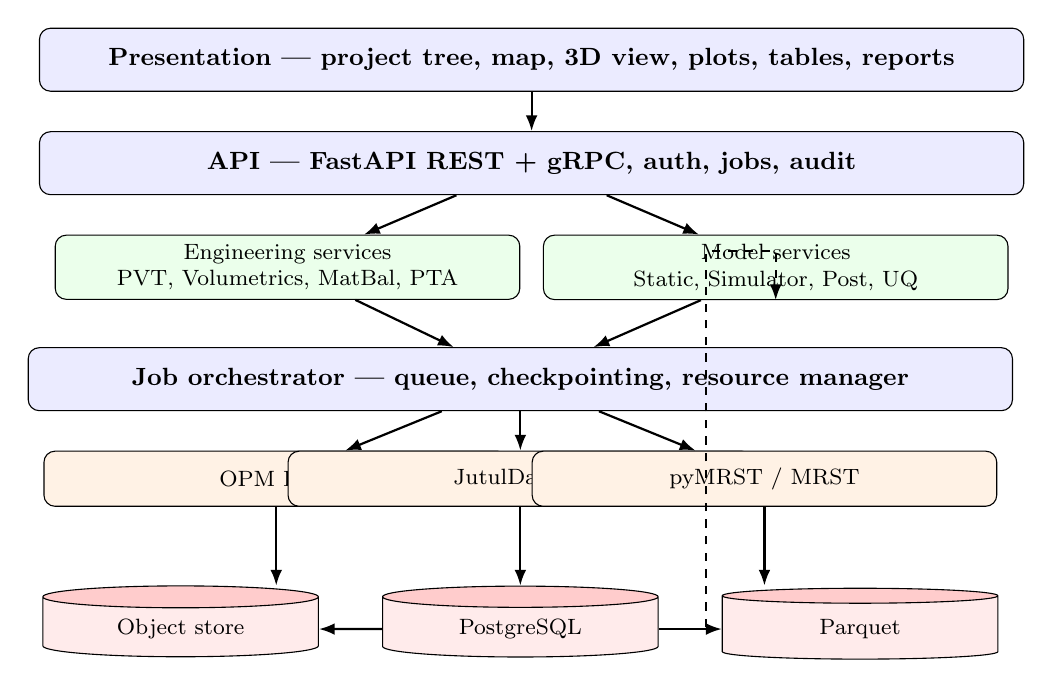
\begin{tikzpicture}[
  node distance=5mm and 8mm,
  layer/.style={draw, rounded corners, minimum width=12.5cm,
                minimum height=0.8cm, align=center, font=\small\bfseries,
                fill=blue!8},
  box/.style={draw, rounded corners, minimum width=5.9cm,
              minimum height=0.7cm, align=center, font=\footnotesize},
  store/.style={draw, cylinder, cylinder uses custom fill,
                cylinder body fill=red!8, cylinder end fill=red!20,
                shape border rotate=90, aspect=0.15, minimum width=3.5cm,
                minimum height=0.9cm, align=center, font=\footnotesize},
  arr/.style={-{Latex[length=2mm]}, thick},
  darr/.style={-{Latex[length=2mm]}, thick, dashed}
]
% Layers
\node[layer] (ui) {Presentation --- project tree, map, 3D view, plots, tables, reports};
\node[layer, below=of ui] (api) {API --- FastAPI REST + gRPC, auth, jobs, audit};
\node[box, below=of api, xshift=-3.1cm, fill=green!8] (dom1) {Engineering services\\PVT, Volumetrics, MatBal, PTA};
\node[box, below=of api, xshift=3.1cm, fill=green!8] (dom2) {Model services\\Static, Simulator, Post, UQ};
\node[layer, below=of dom1.south east, yshift=-0.1cm] (orch) {Job orchestrator --- queue, checkpointing, resource manager};
\node[box, below=of orch, xshift=-3.1cm, fill=orange!10] (ext1) {OPM Flow};
\node[box, below=of orch, xshift=0cm, fill=orange!10] (ext2) {JutulDarcy.jl};
\node[box, below=of orch, xshift=3.1cm, fill=orange!10] (ext3) {pyMRST / MRST};
\node[store, below=of ext2, yshift=-0.5cm] (pg) {PostgreSQL};
\node[store, right=of pg] (parquet) {Parquet};
\node[store, left=of pg] (obj) {Object store};

% Arrows
\draw[arr] (ui) -- (api);
\draw[arr] (api) -- (dom1);
\draw[arr] (api) -- (dom2);
\draw[arr] (dom1) -- (orch);
\draw[arr] (dom2) -- (orch);
\draw[arr] (orch) -- (ext1);
\draw[arr] (orch) -- (ext2);
\draw[arr] (orch) -- (ext3);
\draw[arr] (ext1) -- (ext1 |- pg.north);
\draw[arr] (ext2) -- (pg);
\draw[arr] (ext3) -- (ext3 |- pg.north);
\draw[arr] (pg) -- (parquet);
\draw[arr] (pg) -- (obj);
\draw[darr] (pg.east) ++(0.2,0) -- ++(0.4,0) |- ++(0,4.8) -| (dom2.south);
\end{tikzpicture}
\caption{Layered architecture of the \petro reservoir module. Blue bands are
framework layers; green are domain services; orange are external engines;
red are storage backends. Dashed arrow is the results feedback path.}
\label{fig:arch}
\end{figure}

\subsection{Layer responsibilities}

\begin{longtable}{@{}p{3.1cm}p{11.5cm}@{}}
\toprule
\textbf{Layer} & \textbf{Responsibilities and constraints}\\
\midrule
\endhead
Presentation & Browser or desktop shell. Reads only the public API. No direct
database access. Handles only display concerns; long-running work is always a
job.\\
\midrule
API & FastAPI/gRPC endpoints. Handles authentication, authorisation,
request validation, job submission, result streaming and audit logging. Holds
no engineering logic.\\
\midrule
Domain services & Pure engineering and scientific logic. Each service is a
Python package with a typed interface. Deterministic, unit-safe, side-effect
free except for writing to storage.\\
\midrule
Job orchestrator & Schedules and monitors simulation runs. Owns the queue,
resource allocation, checkpointing, and the \code{Run} state machine.\\
\midrule
External engines & OPM Flow, JutulDarcy, MRST. Invoked as subprocesses or
workers. Never share an address space with \petro itself.\\
\midrule
Storage & PostgreSQL for entities and provenance; Parquet for arrays and time
series; object store for decks, grids and 3D results.\\
\bottomrule
\end{longtable}

\subsection{The package structure}
\begin{lstlisting}[style=txt, caption={Repository layout for the reservoir module.}]
petrolumen/
  pyproject.toml
  src/petrolumen/
    core/
      units.py          # pint registry, canonical SI
      schema.py         # pydantic base models
      errors.py         # domain exceptions
      provenance.py     # environment, engine and deck hashing
      audit.py          # append-only audit log client
    reservoir/
      fluids/
        correlations.py # Standing, Vazquez-Beggs, etc.
        provider.py     # FluidProvider protocol + implementations
        labmatch.py     # lab data fitting
      volumetrics/
        ooip.py
        drive_indices.py
        recovery.py
      matbal/
        havlena_odeh.py
        aquifer.py
      pta/
        loader.py
        derivative.py
        models.py       # radial, fractured, horizontal
        interpret.py
      static/
        grids.py        # Petres wrappers
        geostats.py     # GeostatsPy wrappers
        upscaling.py
        resqml_io.py    # resqpy wrappers
      sim/
        engines/
          base.py       # EnginePlugin protocol
          opm_flow.py
          jutuldarcy.py
          pymrst.py
        deck.py         # Eclipse deck writer
        parse.py        # SMSPEC/UNSMRY/EGRID/UNRST parsers
        scheduler.py
      post/
        summary.py
        threed.py
        plots.py
        forecast.py
      uncertainty/
        samplers.py     # SALib wrappers
        surrogate.py    # scikit-learn wrappers
        hm.py           # assisted history matching
    api/
      routers/
      schemas/
      auth/
    jobs/
      queue.py
      workers.py
      backends/         # local, slurm, kubernetes
  tests/
    unit/
    integration/
    benchmarks/         # SPE1, SPE9, SPE10, Norne fixtures
  docs/
    physics/            # equation references
    api/
    user-guide/
  plugins/
    examples/
\end{lstlisting}

\subsection{Dependency rules}
\begin{itemize}[leftmargin=1.4em]
  \item \code{core} depends on no other \petro package.
  \item Domain services depend on \code{core} and external libraries only.
  \item \code{api} depends on \code{core} and domain services.
  \item \code{jobs} depends on \code{core} and \code{sim.engines.base}.
  \item No package imports an engine implementation directly; only the protocol.
  \item No package writes to storage outside a repository interface defined in
        \code{core}.
\end{itemize}

% ==================================================================
\section{Domain Data Model}
% ==================================================================

\subsection{Entity-relationship overview}

\begin{figure}[htbp]
\centering
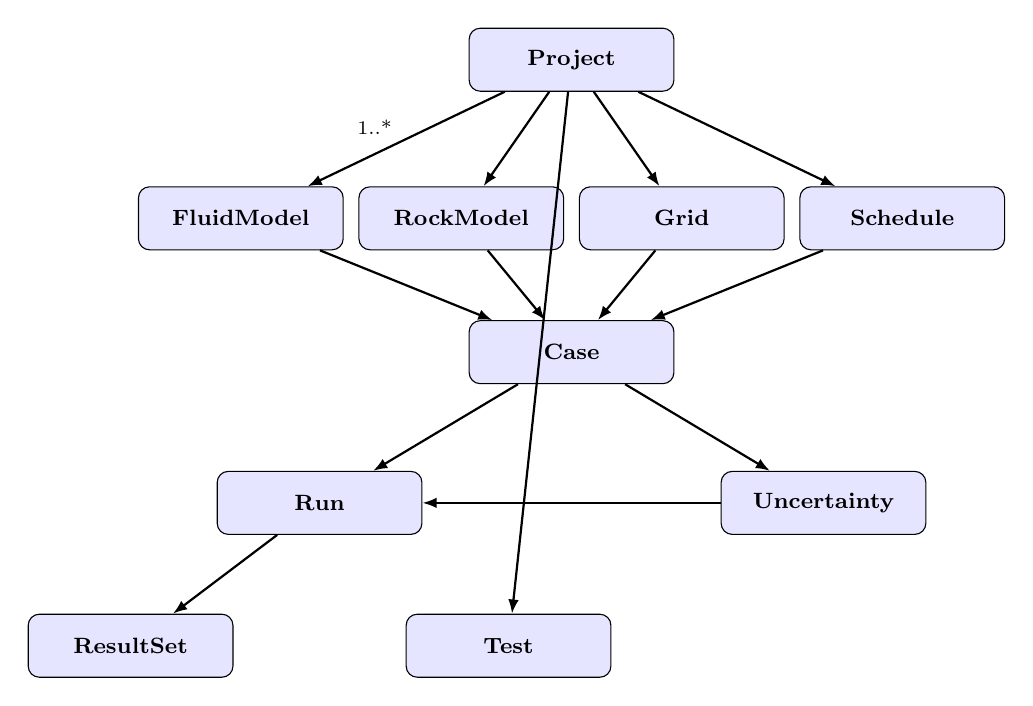
\begin{tikzpicture}[
  entity/.style={draw, rounded corners, minimum width=2.6cm,
                 minimum height=0.8cm, align=center, font=\footnotesize\bfseries,
                 fill=blue!10},
  rel/.style={-{Latex[length=1.8mm]}, thick},
  lbl/.style={font=\scriptsize, fill=white, inner sep=1pt}
]
\node[entity] (proj) {Project};
\node[entity, below=1.2cm of proj, xshift=-4.2cm] (fluid) {FluidModel};
\node[entity, below=1.2cm of proj, xshift=-1.4cm] (rock) {RockModel};
\node[entity, below=1.2cm of proj, xshift=1.4cm] (grid) {Grid};
\node[entity, below=1.2cm of proj, xshift=4.2cm] (sched) {Schedule};
\node[entity, below=2.9cm of proj] (case) {Case};
\node[entity, below=1.1cm of case, xshift=-3.2cm] (run) {Run};
\node[entity, below=1.1cm of case, xshift=3.2cm] (uq) {Uncertainty};
\node[entity, below=1.0cm of run, xshift=-2.4cm] (res) {ResultSet};
\node[entity, below=1.0cm of run, xshift=2.4cm] (test) {Test};

\draw[rel] (proj) -- (fluid); \node[lbl] at ($(proj)!.5!(fluid)+(-0.4,0.15)$) {1..*};
\draw[rel] (proj) -- (rock);
\draw[rel] (proj) -- (grid);
\draw[rel] (proj) -- (sched);
\draw[rel] (grid) -- (case);
\draw[rel] (fluid) -- (case);
\draw[rel] (rock) -- (case);
\draw[rel] (sched) -- (case);
\draw[rel] (case) -- (run);
\draw[rel] (run) -- (res);
\draw[rel] (proj) -- (test);
\draw[rel] (case) -- (uq);
\draw[rel] (uq) -- (run);
\end{tikzpicture}
\caption{Core entity relationships in the reservoir module.}
\label{fig:er}
\end{figure}

\subsection{PostgreSQL DDL (excerpt)}

\begin{lstlisting}[style=sql, caption={Selected DDL for the reservoir module.}]
CREATE SCHEMA reservoir;

CREATE TABLE reservoir.project (
    id           UUID PRIMARY KEY DEFAULT gen_random_uuid(),
    name         TEXT NOT NULL,
    crs          TEXT NOT NULL DEFAULT 'EPSG:4326',
    units        TEXT NOT NULL DEFAULT 'SI',
    owner_id     UUID NOT NULL,
    created_at   TIMESTAMPTZ NOT NULL DEFAULT now(),
    updated_at   TIMESTAMPTZ NOT NULL DEFAULT now(),
    tags         TEXT[],
    UNIQUE (owner_id, name)
);

CREATE TABLE reservoir.fluid_model (
    id           UUID PRIMARY KEY DEFAULT gen_random_uuid(),
    project_id   UUID NOT NULL REFERENCES reservoir.project(id) ON DELETE CASCADE,
    name         TEXT NOT NULL,
    kind         TEXT NOT NULL CHECK (kind IN ('black_oil','compositional')),
    component_table  JSONB,
    correlations     JSONB,
    lab_source       TEXT,
    version      INT NOT NULL DEFAULT 1,
    created_at   TIMESTAMPTZ NOT NULL DEFAULT now(),
    UNIQUE (project_id, name, version)
);

CREATE TABLE reservoir.grid (
    id           UUID PRIMARY KEY DEFAULT gen_random_uuid(),
    project_id   UUID NOT NULL REFERENCES reservoir.project(id) ON DELETE CASCADE,
    name         TEXT NOT NULL,
    format       TEXT NOT NULL CHECK (format IN ('corner_point','cpg','resqml')),
    dims         INT[] NOT NULL,
    active_mask  BYTEA,
    data_uri     TEXT NOT NULL,
    parent_grid  UUID REFERENCES reservoir.grid(id),
    UNIQUE (project_id, name)
);

CREATE TABLE reservoir.case (
    id           UUID PRIMARY KEY DEFAULT gen_random_uuid(),
    project_id   UUID NOT NULL REFERENCES reservoir.project(id) ON DELETE CASCADE,
    name         TEXT NOT NULL,
    grid_id      UUID REFERENCES reservoir.grid(id),
    fluid_id     UUID REFERENCES reservoir.fluid_model(id),
    rock_id      UUID REFERENCES reservoir.rock_model(id),
    schedule_id  UUID REFERENCES reservoir.schedule(id),
    engine       TEXT NOT NULL,
    solver_opts  JSONB NOT NULL DEFAULT '{}'::jsonb,
    parent_case  UUID REFERENCES reservoir.case(id),
    created_at   TIMESTAMPTZ NOT NULL DEFAULT now(),
    UNIQUE (project_id, name)
);

CREATE TABLE reservoir.run (
    id              UUID PRIMARY KEY DEFAULT gen_random_uuid(),
    case_id         UUID NOT NULL REFERENCES reservoir.case(id) ON DELETE CASCADE,
    deck_hash       CHAR(64) NOT NULL,
    engine_version  TEXT NOT NULL,
    env_hash        CHAR(64) NOT NULL,
    status          TEXT NOT NULL CHECK (status IN
                     ('queued','running','succeeded','failed','cancelled')),
    started_at      TIMESTAMPTZ,
    finished_at     TIMESTAMPTZ,
    exit_code       INT,
    log_uri         TEXT,
    result_uri      TEXT,
    operator_id     UUID NOT NULL
);

CREATE INDEX ON reservoir.run (case_id);
CREATE INDEX ON reservoir.run (status) WHERE status IN ('queued','running');

CREATE TABLE reservoir.result_set (
    id           UUID PRIMARY KEY DEFAULT gen_random_uuid(),
    run_id       UUID NOT NULL REFERENCES reservoir.run(id) ON DELETE CASCADE,
    kind         TEXT NOT NULL CHECK (kind IN ('summary','grid','time_series')),
    variables    TEXT[],
    time_range   TSRANGE,
    data_uri     TEXT NOT NULL
);

CREATE TABLE reservoir.audit_log (
    id           BIGSERIAL PRIMARY KEY,
    at           TIMESTAMPTZ NOT NULL DEFAULT now(),
    actor_id     UUID NOT NULL,
    project_id   UUID,
    action       TEXT NOT NULL,
    payload      JSONB NOT NULL
);
\end{lstlisting}

\subsection{Typed domain objects}

\begin{lstlisting}[caption={Core pydantic models.}]
from __future__ import annotations
from datetime import datetime
from enum import Enum
from typing import Optional
from uuid import UUID
import pint
from pydantic import BaseModel, Field, field_validator

ureg = pint.UnitRegistry()
Q = ureg.Quantity

class Engine(str, Enum):
    OPM_FLOW = "opm_flow"
    JUTULDARCY = "jutuldarcy"
    PYMRST = "pymrst"

class Units(str, Enum):
    SI = "SI"
    FIELD = "FIELD"

class Case(BaseModel):
    id: UUID
    project_id: UUID
    name: str
    grid_id: UUID
    fluid_id: UUID
    rock_id: UUID
    schedule_id: UUID
    engine: Engine = Engine.OPM_FLOW
    solver: dict = Field(default_factory=dict)
    parent_case: Optional[UUID] = None
    created_at: datetime

class RunStatus(str, Enum):
    QUEUED = "queued"
    RUNNING = "running"
    SUCCEEDED = "succeeded"
    FAILED = "failed"
    CANCELLED = "cancelled"

class Run(BaseModel):
    id: UUID
    case_id: UUID
    deck_hash: str = Field(min_length=64, max_length=64)
    engine_version: str
    env_hash: str = Field(min_length=64, max_length=64)
    status: RunStatus
    started_at: Optional[datetime]
    finished_at: Optional[datetime]
    exit_code: Optional[int]
    log_uri: Optional[str]
    result_uri: Optional[str]
    operator_id: UUID

class PressurePoint(BaseModel):
    t: float
    p: float
    q: Optional[float] = None

    @field_validator("t", "p")
    @classmethod
    def non_negative(cls, v: float) -> float:
        if v < 0:
            raise ValueError("time and pressure must be non-negative")
        return v

class Test(BaseModel):
    id: UUID
    well_id: UUID
    points: list[PressurePoint]
    interpretation: Optional[dict] = None
\end{lstlisting}

\subsection{Storage partition}

\begin{longtable}{@{}p{3.0cm}p{5.5cm}p{6.1cm}@{}}
\toprule
\textbf{Store} & \textbf{Content} & \textbf{Rationale}\\
\midrule
\endhead
PostgreSQL & Entities in the DDL above, audit log, provenance records, user metadata & Transactional, queryable, joinable; small enough to keep in a single database\\
\midrule
Parquet & Summary vectors, per-well time series, ensemble result arrays & Columnar, compressed, fast to scan; partition by \code{run\_id} and \code{variable}\\
\midrule
Object store & Eclipse decks, RESQML/HDF5 models, restart files, 3D arrays & Large, immutable, content-addressed by hash\\
\bottomrule
\end{longtable}

% ==================================================================
\section{Public API}
% ==================================================================

\subsection{Style}
The API is REST (JSON) for control-plane operations, gRPC for streaming
(time series, ensemble results) and plain HTTP for file download. All endpoints
are versioned under \code{/v1/}.

\subsection{Endpoints (excerpt)}

\begin{longtable}{@{}p{1.4cm}p{4.6cm}p{8.2cm}@{}}
\toprule
\textbf{Verb} & \textbf{Path} & \textbf{Purpose}\\
\midrule
\endhead
GET    & \code{/v1/projects} & List projects visible to the caller\\
POST   & \code{/v1/projects} & Create project\\
POST   & \code{/v1/projects/\{id\}/fluids} & Upload or build a fluid model\\
POST   & \code{/v1/projects/\{id\}/grids} & Upload a grid (RESQML or GRDECL)\\
POST   & \code{/v1/projects/\{id\}/tests} & Upload a pressure transient test\\
POST   & \code{/v1/projects/\{id\}/tests/\{tid\}/interpret} & Run PTA interpretation\\
POST   & \code{/v1/projects/\{id\}/cases} & Create simulation case\\
POST   & \code{/v1/cases/\{id\}/runs} & Submit run (returns run id)\\
GET    & \code{/v1/runs/\{id\}} & Poll status\\
GET    & \code{/v1/runs/\{id\}/stream} & gRPC stream of live log and progress\\
GET    & \code{/v1/runs/\{id\}/results} & List result sets\\
GET    & \code{/v1/results/\{id\}/summary} & Download summary vectors as Parquet\\
POST   & \code{/v1/projects/\{id\}/uncertainty} & Launch an ensemble\\
POST   & \code{/v1/projects/\{id\}/hm} & Launch assisted history matching\\
\bottomrule
\end{longtable}

\subsection{Example: create a case and run it}

\begin{lstlisting}[caption={End-to-end API usage from Python.}]
import httpx

BASE = "https://petrolumen.local/v1"
auth = {"Authorization": "Bearer <token>"}

case = httpx.post(f"{BASE}/projects/{proj}/cases", headers=auth, json={
    "name": "spe1-base",
    "grid_id": grid_id,
    "fluid_id": fluid_id,
    "rock_id": rock_id,
    "schedule_id": schedule_id,
    "engine": "opm_flow",
    "solver": {"threads": 8, "max_timestep_days": 30},
}).json()

run = httpx.post(f"{BASE}/cases/{case['id']}/runs", headers=auth).json()

while True:
    status = httpx.get(f"{BASE}/runs/{run['id']}", headers=auth).json()
    if status["status"] in {"succeeded", "failed", "cancelled"}:
        break
    httpx.sleep(5)

assert status["status"] == "succeeded", status["exit_code"]
summary = httpx.get(
    f"{BASE}/results/{status['result_id']}/summary",
    headers=auth, params={"variables": ["FOPR", "FOPT", "WBHP:PROD"]}
)
open("spe1-summary.parquet", "wb").write(summary.content)
\end{lstlisting}

% ==================================================================
\section{The Free Tool Stack}
% ==================================================================

\subsection{Complete mapping}

\begin{longtable}{@{}p{2.4cm}p{2.9cm}p{1.9cm}p{1.7cm}p{4.5cm}@{}}
\toprule
\textbf{Concern} & \textbf{Tool} & \textbf{Licence} & \textbf{Version} & \textbf{Role}\\
\midrule
\endhead
Simulator (CPU)     & OPM Flow        & OSL-3.0/GPL & $\geq$2024.04 & Full-field black-oil and compositional\\
Simulator (fast)    & JutulDarcy.jl   & MIT         & $\geq$0.4     & Prototyping, differentiable workflows\\
Simulator (research)& MRST / pyMRST   & GPL-3.0     & $\geq$2023b   & Custom discretisations, teaching\\
Grids               & Petres          & LGPL        & $\geq$1.3     & Corner-point grids, GRDECL I/O\\
Model exchange      & resqpy          & Apache-2.0  & $\geq$3.14    & RESQML read/write\\
Geostatistics       & GeostatsPy      & MIT         & latest        & Kriging, SGS, property models\\
PVT                 & pyResToolbox    & GPL-3.0     & latest        & Fluid correlations\\
General calcs       & PetroCalc       & MIT         & $\geq$1.3     & Volumetrics, IPR, economics\\
Well testing        & welltest-pta    & MIT         & latest        & Derivative, Horner, fitting\\
Well testing (auto) & pta-learn       & MIT         & latest        & Transient / flow regime detection\\
Nodal               & pynodal         & MIT         & latest        & IPR/VLP\\
Arrays              & NumPy, SciPy    & BSD         & stable        & Linear algebra, ODE/PDE\\
Tabular             & pandas, xarray  & BSD/Apache  & stable        & Time series, gridded results\\
3D viz (in-app)     & PyVista         & MIT         & stable        & In-app 3D grid rendering\\
3D viz (external)   & ResInsight      & GPL-3.0     & $\geq$2024.04 & Optional large-model viewer\\
2D plots            & matplotlib      & PSF         & stable        & Standard engineering plots\\
Uncertainty         & SALib           & MIT         & stable        & Sampling, sensitivity\\
Surrogates          & scikit-learn    & BSD         & stable        & RF, GP for surrogate models\\
Units               & pint            & BSD         & stable        & Unit-safe quantities\\
Schema              & pydantic        & MIT         & $\geq$2.6     & Typed domain objects\\
API                 & FastAPI         & MIT         & stable        & HTTP/gRPC service layer\\
Queue               & Celery or RQ    & BSD         & stable        & Job queue\\
Database            & PostgreSQL      & PostgreSQL  & $\geq$15      & Metadata, provenance\\
Compression         & pyarrow         & Apache-2.0  & stable        & Parquet I/O\\
\bottomrule
\end{longtable}

\subsection{Version pinning policy}
\petro adopts semantic versioning for itself, and pins external dependencies to
\emph{compatible-release} ranges in \code{pyproject.toml}:
\begin{lstlisting}[style=txt, caption={Excerpt of pyproject.toml dependency pinning.}]
[project]
dependencies = [
    "pydantic>=2.6,<3",
    "pint>=0.22,<1",
    "numpy>=1.26,<3",
    "scipy>=1.11,<2",
    "pandas>=2.1,<3",
    "xarray>=2023.10,<2025",
    "pyarrow>=14,<16",
    "fastapi>=0.110,<1",
    "uvicorn>=0.29,<1",
    "celery>=5.3,<6",
    "redis>=5.0,<6",
    "resqpy>=3.14,<4",
    "petres>=1.3,<2",
    "geostatsypy>=0.0.1,<1",
    "pyvista>=0.43,<1",
    "welltest-pta>=0.1,<1",
    "salib>=1.4,<2",
    "scikit-learn>=1.4,<2",
]

[project.optional-dependencies]
gpl-engines = [
    "pyResToolbox>=0.1,<1",
    "pymrst>=0.1,<1",
]
\end{lstlisting}

\subsection{Licensing strategy}

The dependency graph mixes permissive (MIT/BSD/Apache) and copyleft (GPL)
components. \petro's strategy is:

\begin{longtable}{@{}p{3.3cm}p{4.0cm}p{6.1cm}@{}}
\toprule
\textbf{Licence class} & \textbf{Components} & \textbf{Integration rule}\\
\midrule
\endhead
Permissive & resqpy, Petres, GeostatsPy, welltest-pta, pta-learn, SALib, scikit-learn, pydantic, pint, FastAPI, PyVista, pandas, xarray, PyArrow & Imported directly; safe to link; \petro can be Apache-2.0\\
\midrule
Copyleft & OPM Flow, MRST, pyMRST, ResInsight, pyResToolbox & Invoked as \emph{external processes} or optional extras; never linked into the \petro address space\\
\midrule
Weak copyleft & Petres (LGPL) & Used as a dynamic dependency; \petro itself remains permissively licensed\\
\bottomrule
\end{longtable}

\noindent The operative rule is \textbf{process isolation}: any GPL code that
\petro invokes lives behind a subprocess or network boundary. The
\code{EnginePlugin} protocol is the mechanism that enforces this.

% ==================================================================
\section{Module 1: Core Infrastructure}
% ==================================================================

\subsection{Units}
All physical quantities are \code{pint.Quantity} objects. The canonical internal
unit system is SI, with the following exceptions:
\begin{itemize}[leftmargin=1.4em]
  \item pressure: \si{Pa} (converted to \si{bar} or \si{psi} only at display);
  \item permeability: \si{m^2} (converted to \si{mD} at display);
  \item viscosity: \si{Pa.s} (converted to \si{cP} at display);
  \item volume: \si{m^3} (converted to \si{bbl} or \si{ft^3} at display).
\end{itemize}

\begin{lstlisting}[caption={Unit helper module.}]
import pint
ureg = pint.UnitRegistry()
ureg.define("darcy = 9.869233e-13 * m**2 = D")
ureg.define("millidarcy = 1e-3 * darcy = mD")

def to_display(value: pint.Quantity, unit: str) -> float:
    return value.to(unit).magnitude
\end{lstlisting}

\subsection{Provenance and hashing}

\begin{lstlisting}[caption={Environment and deck hashing.}]
import hashlib, json, os, platform, subprocess, sys
from importlib.metadata import version

def deck_hash(deck_path: str) -> str:
    with open(deck_path, "rb") as f:
        return hashlib.sha256(f.read()).hexdigest()

def engine_version(engine: str) -> str:
    if engine == "opm_flow":
        out = subprocess.check_output(["flow", "--version"], text=True)
        return out.strip().splitlines()[0]
    if engine == "jutuldarcy":
        return version("juliacall")  # or query the Julia env
    return "unknown"

def env_hash() -> str:
    payload = {
        "python": sys.version,
        "platform": platform.platform(),
        "packages": {
            p: version(p)
            for p in ["numpy", "scipy", "pandas", "resqpy", "petres"]
        },
    }
    return hashlib.sha256(
        json.dumps(payload, sort_keys=True).encode()
    ).hexdigest()
\end{lstlisting}

\subsection{Errors}
The domain error hierarchy:
\begin{lstlisting}[caption={Domain exceptions.}]
class PetrolumenError(Exception): ...
class ValidationError(PetrolumenError): ...
class UnitMismatch(ValidationError): ...
class OutOfRangeError(ValidationError): ...
class EngineError(PetrolumenError): ...
class EngineNotAvailable(EngineError): ...
class RunFailed(EngineError): ...
class StorageError(PetrolumenError): ...
\end{lstlisting}

% ==================================================================
\section{Module 2: Fluids and PVT}
% ==================================================================

\subsection{Physics}
The module implements the standard black-oil PVT relationships. Key
correlations implemented in \code{fluids/correlations.py}:

\paragraph{Standing's $R_s$ (gas solubility).}
\begin{equation}
R_s = \gamma_g \left[ \left( \frac{p}{18.2} + 1.4 \right) 10^{0.0125\,\text{API} - 0.00091\,T} \right]^{1.2048}
\end{equation}
where $p$ in psia, $T$ in $^\circ$F, $\gamma_g$ gas specific gravity, API oil
gravity.

\paragraph{Standing's $B_o$ (oil formation volume factor).}
\begin{equation}
B_o = 0.972 + 0.000147 F^{1.175}, \qquad
F = R_s \left( \frac{\gamma_g}{\gamma_o} \right)^{0.5} + 1.25 T
\end{equation}

\paragraph{Vasquez--Beggs $R_s$.}
For $p \le p_b$:
\begin{equation}
R_s = C_1 \gamma_g\, p^{C_2} \exp\!\left[ C_3 \frac{\text{API}}{T + 460} \right]
\end{equation}
with $C_1, C_2, C_3$ depending on whether API $\le 30$ or $> 30$.

\paragraph{Hall--Yarborough $Z$-factor.}
\begin{equation}
Z = \frac{0.06125\, p_r}{Y} \exp\!\left[ -1.2 (1 - 1/T_r)^2 \right]
\end{equation}
where $Y$ solves
\begin{equation}
-0.06125 p_r \frac{\exp[-1.2(1-1/T_r)^2]}{Y} + \frac{Y + Y^2 + Y^3 - Y^4}{(1-Y)^3}
- (14.76/T_r - 9.76/T_r^2 + 4.58/T_r^3) Y^2 \nonumber
+ (90.7/T_r - 242.2/T_r^2 + 42.4/T_r^3) Y^{2.18 + 2.82/T_r} = 0
\end{equation}

\subsection{Implementation}

\begin{lstlisting}[caption={Black-oil PVT table builder.}]
from dataclasses import dataclass
import numpy as np

@dataclass(frozen=True)
class BlackOilTable:
    p: np.ndarray      # psia
    rs: np.ndarray     # scf/STB
    bo: np.ndarray     # RB/STB
    mu_o: np.ndarray   # cP
    bg: np.ndarray     # RB/scf
    mu_g: np.ndarray   # cP
    p_bubble: float

def standing_rs(p, t_f, api, gamma_g):
    x = (p / 18.2 + 1.4) * 10 ** (0.0125 * api - 0.00091 * t_f)
    return gamma_g * np.power(np.maximum(x, 1e-12), 1.2048)

def standing_bo(rs, t_f, api, gamma_g):
    gamma_o = 141.5 / (api + 131.5)
    F = rs * np.sqrt(gamma_g / gamma_o) + 1.25 * t_f
    return 0.972 + 0.000147 * np.power(F, 1.175)

def build_table(p_grid, t_f, api, gamma_g, p_bubble):
    rs = np.where(p_grid <= p_bubble,
                  standing_rs(p_grid, t_f, api, gamma_g),
                  standing_rs(p_bubble, t_f, api, gamma_g))
    bo = np.where(p_grid <= p_bubble,
                  standing_bo(rs, t_f, api, gamma_g),
                  standing_bo(rs, t_f, api, gamma_g) *
                  np.exp(-1.5e-5 * (p_grid - p_bubble)))
    # viscosity via Beggs-Robinson etc. omitted for brevity
    mu_o = np.full_like(p_grid, np.nan)
    bg = np.full_like(p_grid, np.nan)
    mu_g = np.full_like(p_grid, np.nan)
    return BlackOilTable(p_grid, rs, bo, mu_o, bg, mu_g, p_bubble)
\end{lstlisting}

\subsection{Provider protocol}

\begin{lstlisting}[caption={Fluid provider interface.}]
from typing import Protocol

class FluidProvider(Protocol):
    name: str
    kind: str

    def rs(self, p: float, t: float) -> float: ...
    def bo(self, p: float, t: float) -> float: ...
    def mu_o(self, p: float, t: float) -> float: ...
    def bg(self, p: float, t: float) -> float: ...
    def mu_g(self, p: float, t: float) -> float: ...
    def to_black_oil_table(
        self, p_grid: list[float], t: float
    ) -> "BlackOilTable": ...
\end{lstlisting}

\subsection{Guardrails}
\begin{itemize}[leftmargin=1.4em]
  \item Reject inputs outside a correlation's fitted range; raise
        \code{OutOfRangeError} with the specific bound violated.
  \item Record the exact correlation name and version used in
        \code{fluid\_model.correlations}.
  \item If lab data is present, fit the correlations to it and store both the
        raw lab data and the fitted parameters as separate, versioned records.
  \item Provide a monotonically non-decreasing $R_s$, $B_o$ sanity check on
        table construction; warn if violated.
\end{itemize}

% ==================================================================
\section{Module 3: Volumetrics and Material Balance}
% ==================================================================

\subsection{Volumetrics}
\begin{equation}
N = \frac{7758 \, A \, h \, \phi \, (1 - S_w)}{B_{oi}} \quad \text{(STB)}
\end{equation}
where $A$ in acres, $h$ in ft, $\phi$ fraction, $S_w$ fraction, $B_{oi}$ RB/STB.

\subsection{Material balance (general form)}
\begin{equation}
N_p [B_o + (R_p - R_s) B_g] + W_p B_w =
N [B_o - B_{oi} + (R_{si} - R_s) B_g + m B_{oi} (B_g/B_{gi} - 1)]
+ (W_e + W_{inj} - W_p) B_w + G_{inj} B_{ig}
\end{equation}

\subsection{Havlena--Odeh straight-line form}
For a solution-gas-drive reservoir with no water influx, no gas cap, and no
injection:
\begin{equation}
\frac{N_p B_o}{B_o - B_{oi}} = N + \frac{R_{si} - R_s}{B_o - B_{oi}} N_p
\end{equation}
Plotting $N_p B_o / (B_o - B_{oi})$ against $(R_{si} - R_s) N_p / (B_o - B_{oi})$
yields intercept $N$ and slope equal to $N$.

With water influx, the form generalises to include $W_e$ as an additional term;
a separate aquifer model (Fetkovich or van Everdingen--Hurst) is required to
close the equation.

\subsection{Implementation}

\begin{lstlisting}[caption={Havlena-Odeh analysis.}]
import numpy as np

def havlena_odeh(np_, rs, bo, rsi, boi):
    y = np_.sum(axis=0) * bo / (bo - boi)
    x = (rsi - rs) * np_.sum(axis=0) / (bo - boi)
    A = np.vstack([x, np.ones_like(x)]).T
    slope, intercept = np.linalg.lstsq(A, y, rcond=None)[0]
    return {"N": intercept, "slope": slope,
            "residuals": y - (slope * x + intercept)}
\end{lstlisting}

\subsection{Aquifer models}
\begin{itemize}[leftmargin=1.4em]
  \item \textbf{Fetkovich:} pseudo-steady-state, useful for small aquifers,
        closed-form \code{We = We\_max * (1 - exp(-J * (pi - p) * t / We\_max))}
        with $J$ aquifer productivity and $p_i$ initial pressure.
  \item \textbf{van Everdingen--Hurst:} transient, requires dimensionless
        aquifer functions $W_{eD}(t_D)$ for radial or linear geometry.
  \item \textbf{Carter--Tracy:} efficient for simulation-style forecasting.
\end{itemize}

\subsection{Guardrails}
\begin{itemize}[leftmargin=1.4em]
  \item Unit checks on \emph{every} term of the material balance; a mismatch is
        a hard error, not a warning.
  \item Havlena--Odeh is only valid when a straight line actually fits;
        the module must report $R^2$ and refuse to draw a line if $R^2 < 0.9$.
  \item Aquifer selection is an engineering decision, not an automatic one;
        the UI must require an explicit model choice.
\end{itemize}

% ==================================================================
\section{Module 4: Pressure Transient Analysis}
% ==================================================================

\subsection{Radial flow equation}
The diffusivity equation for a single-phase, slightly compressible fluid in a
radial reservoir:
\begin{equation}
\frac{1}{r} \frac{\partial}{\partial r}\left( r \frac{\partial p}{\partial r} \right)
= \frac{\phi \mu c_t}{k} \frac{\partial p}{\partial t}
\end{equation}

The line-source solution (exponential integral, $E_i$):
\begin{equation}
p_{wf}(t) = p_i - \frac{q B \mu}{4 \pi k h} E_1\!\left( \frac{\phi \mu c_t r_w^2}{4 k t} \right)
\end{equation}

For large $t$ (the semilog straight line):
\begin{equation}
p_{wf} = p_i - \frac{162.6 \, q B \mu}{k h} \left[ \log_{10} t + \log_{10}\!\left(\frac{k}{\phi \mu c_t r_w^2}\right) - 3.23 + 0.87 s \right]
\end{equation}

\subsection{Bourdet derivative}
\begin{equation}
p' = \frac{\dd p}{\dd \ln t} \approx \frac{\Delta p_1 \ln(t_2/t_0) + \Delta p_2 \ln(t_0/t_1)}{\ln(t_2/t_0) \ln(t_2/t_1) \ln(t_1/t_0)}
\end{equation}
for a three-point window $(t_0, t_1, t_2)$; window selection is the key
engineering decision. The module must expose the $L$-parameter (window width)
as a knob and show the derivative response interactively.

\subsection{Horner plot}
\begin{equation}
p_{ws} = p_i - \frac{162.6 \, q B \mu}{k h} \log_{10}\!\left( \frac{t_p + \Delta t}{\Delta t} \right)
\end{equation}

Permeability from slope $m$:
\begin{equation}
k = \frac{162.6 \, q B \mu}{m h}
\end{equation}
Skin from intercept at $\Delta t \to \infty$:
\begin{equation}
s = 1.151 \left[ \frac{p_1 - p_{wf}}{m} - \log_{10}\!\left(\frac{k}{\phi \mu c_t r_w^2}\right) + 3.23 \right]
\end{equation}

\subsection{Models implemented}

\begin{longtable}{@{}p{3.0cm}p{5.5cm}p{6.0cm}@{}}
\toprule
\textbf{Model} & \textbf{Signature on log--log} & \textbf{Parameters}\\
\midrule
\endhead
Radial homogeneous & Unit-slope WBS $\to$ 0.5-slope radial $\to$ boundary & $k, s, C$\\
Fractured (infinite conductivity) & Unit-slope bilinear then linear & $x_f, k, s$\\
Fractured (finite conductivity) & Bilinear $\to$ linear $\to$ radial & $x_f, C_{fD}, k, s$\\
Horizontal well & Early radial $\to$ linear $\to$ late radial & $k_h, k_v, L, s$\\
Dual porosity & Valley between two plateaus & $\omega, \lambda, k, s$\\
Sealing fault & Doubled slope on derivative & distance $L$\\
Constant-pressure boundary & Declining derivative & distance $L$\\
\bottomrule
\end{longtable}

\subsection{Implementation}

\begin{lstlisting}[caption={Bourdet derivative with configurable window.}]
import numpy as np

def bourdet_derivative(t, p, L=0.1):
    """L is the logarithmic window width. Bourdet recommends L = 0.1-0.2."""
    t = np.asarray(t, dtype=float)
    p = np.asarray(p, dtype=float)
    logt = np.log(t)
    n = len(t)
    dpdln = np.full(n, np.nan)
    for i in range(1, n - 1):
        # select the nearest point to the left of t_i * exp(-L)
        left = i - 1
        while left > 0 and logt[i] - logt[left] < L:
            left -= 1
        right = i + 1
        while right < n - 1 and logt[right] - logt[i] < L:
            right += 1
        dl = logt[right] - logt[left]
        if dl > 0:
            dpdln[i] = (
                p[i] - p[left]
            ) / (logt[i] - logt[left]) * (logt[right] - logt[i]) / dl \
            + (p[right] - p[i]) / (logt[right] - logt[i]) * (logt[i] - logt[left]) / dl
    return dpdln
\end{lstlisting}

\subsection{Guardrails}
\begin{itemize}[leftmargin=1.4em]
  \item Require a QC step: downsampling, outlier removal, and rate alignment
        before any derivative is computed.
  \item Show the raw data, the derivative, and the chosen model together; never
        present a fit without the diagnostic plot.
  \item Reject fits with $R^2 < 0.85$ on the fitted segment and explain why.
  \item For build-up tests, warn if the producing time is short relative to the
        shut-in duration ($t_p < 3 \Delta t_{max}$).
\end{itemize}

% ==================================================================
\section{Module 5: Static Modelling}
% ==================================================================

\subsection{Grid handling}
\code{static/grids.py} wraps Petres to:
\begin{itemize}[leftmargin=1.4em]
  \item read and write \code{.GRDECL} (corner-point) grids;
  \item expose cell centres, dimensions and active mask as numpy arrays;
  \item support grid refinement and coarsening for upscaling;
  \item validate geometry (no negative volumes, no inverted cells, consistent
        $z$ direction).
\end{itemize}

\subsection{Geostatistics}
Implemented in \code{static/geostats.py} via GeostatsPy:
\begin{itemize}[leftmargin=1.4em]
  \item variogram fitting (spherical, exponential, Gaussian, power);
  \item ordinary kriging with anisotropic ranges;
  \item sequential Gaussian simulation for property realisations;
  \item facies simulation via indicator kriging or truncated Gaussian.
\end{itemize}

\paragraph{Ordinary kriging.}
Given $n$ samples $z(\mathbf{u}_\alpha)$, the kriging estimate at $\mathbf{u}$ is
\begin{equation}
z^*(\mathbf{u}) = \sum_{\alpha=1}^{n} \lambda_\alpha z(\mathbf{u}_\alpha)
\end{equation}
with weights $\lambda_\alpha$ solving the kriging system
\begin{equation}
\sum_{\beta=1}^{n} \lambda_\beta \, C(\mathbf{u}_\alpha - \mathbf{u}_\beta)
+ \mu = C(\mathbf{u}_\alpha - \mathbf{u}), \quad \alpha = 1, \dots, n
\end{equation}
and $\sum \lambda_\alpha = 1$.

\subsection{Upscaling}
Two main approaches:
\begin{itemize}[leftmargin=1.4em]
  \item \textbf{Flow-based upscaling:} solve single-phase flow on the fine grid
        with unit pressure gradient, compute effective permeability from total
        flux, repeat for each direction.
  \item \textbf{Power-law averaging:} $\bar k = (\frac{1}{V} \int k^p \, dV)^{1/p}$
        with $p \in [-1, 1]$; $p=1$ is arithmetic, $p=-1$ is harmonic.
\end{itemize}
The module must offer both and store the chosen upscaling parameters in
provenance.

\subsection{RESQML interoperability}
\code{static/resqml\_io.py} uses resqpy to:
\begin{itemize}[leftmargin=1.4em]
  \item open, validate and query RESQML 2.0/2.2 models;
  \item extract the grid, properties and horizons into \petro's data model;
  \item write a \petro project back to RESQML for external tools.
\end{itemize}

\subsection{Guardrails}
\begin{itemize}[leftmargin=1.4em]
  \item Coordinate reference systems: every grid must declare a CRS; mismatches
        across imported data are a hard error.
  \item Property ranges: reject porosities outside $[0, 1]$, saturations
        outside $[0, 1]$, permeabilities outside $[10^{-8}, 10^{4}]$ m$^2$ by
        default (configurable).
  \item Upscaling must preserve total pore volume and bulk volume within 1\%.
\end{itemize